\documentclass[10pt, a4paper]{article}
\usepackage{../../../style}

\begin{document}
		
\lhead{Планиметрия}
\rhead{Школа <<Симметрия>>}

\section{Треугольники}
\subsection{Признаки равенства треугольников}
	\begin{enumerate}
		\item \source{Гордин Р.К. Планиметрия, №1.40} Медиана $AM$ треугольника $ABC$ перпендикулярна его биссектрисе $BK$. Найдите $AB$, если $BC = 12$.
		\item \source{Гордин Р.К. Планиметрия, №1.41} Прямая,  проведенная  через  вершину  $A$  треугольника $ABC$ перпендикулярно его медиане $BD$, 
делит эту медиану пополам. Найдите отношение сторон $AB$ и $AC$.
		\item \source{Гордин Р.К. Планиметрия, №1.42} $x+4=9$

		\item \source{Гордин Р.К. Планиметрия, №1.34} Докажите, что в равных треугольниках соответствующие медианы равны.
		\item \source{Гордин Р.К. Планиметрия, №1.35} Какое из чисел отмечено на координатной прямой точкой $A$?
\begin{center}
	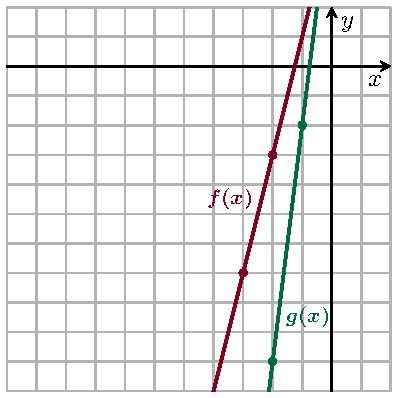
\includegraphics[align=t,]{graphs/graph_5/graph_5}
\end{center}

\textit{В ответе укажите номер правильного варианта.}
\begin{multicols}{4}
	\begin{enumerate}[label=\arabic*)]
		\item $\sqrt{4}$
		\item $\sqrt{1}$
		\item $\sqrt{2}$
		\item $\sqrt{5}$
	\end{enumerate}
\end{multicols}
		\item \source{Гордин Р.К. Планиметрия, №1.37} \setnumber{6} \setanswer{4}
\begin{ex}
	Какому промежутку принадлежит число $\sqrt{55}$?
	
	\selectanswer
	\begin{multicols}{4}
		\begin{enumerate}[label=\arabic*)]
			\item $[4;5]$
			\item $[5;6]$
			\item $[6;7]$
			\item $[7;8]$
		\end{enumerate}
	\end{multicols}
\end{ex}
		\item \source{Гордин Р.К. Планиметрия, №1.38} Какому промежутку принадлежит число $\sqrt{37}$?

\textit{В ответе укажите номер правильного варианта.}
\begin{multicols}{4}
	\begin{enumerate}[label=\arabic*)]
		\item $[4;5]$
		\item $[3;4]$
		\item $[6;7]$
		\item $[2;3]$
	\end{enumerate}
\end{multicols}
		\item \source{Гордин Р.К. Планиметрия, №1.46} В треугольнике $ABC$ медиана $AM$ продолжена за точку $M$ на расстояние, равное $AM$. Найдите расстояние от полученной точки до вершин $B$ и $C$, если $AB = 7$, $AC = 11$.
		\item \source{Гордин Р.К. Планиметрия, №1.47} Какому промежутку принадлежит число $3\sqrt{5}$?

\textit{В ответе укажите номер правильного варианта.}
\begin{multicols}{4}
	\begin{enumerate}[label=\arabic*)]
		\item $[3;4]$
		\item $[5;6]$
		\item $[7;8]$
		\item $[6;7]$
	\end{enumerate}
\end{multicols}
		\item \source{Гордин Р.К. Планиметрия, №1.50} $x+4=9$

		\item \source{Гордин Р.К. Планиметрия, №1.51} \setnumber{11} \setanswer{}
\begin{ex}
	Какому промежутку принадлежит число $3\sqrt{10}$?
	
	\selectanswer
	\begin{multicols}{4}
		\begin{enumerate}[label=\arabic*)]
			\item $[9;10]$
			\item $[10;11]$
			\item $[6;7]$
			\item $[8;9]$
		\end{enumerate}
	\end{multicols}
\end{ex}
		\item \source{Гордин Р.К. Планиметрия, №1.52} Две различные окружности пересекаются в точках $A$ и $B$. Докажите, что прямая, проходящая через центры окружностей, делит отрезок $AB$ пополам и перпендикулярна ему.
		\item \source{Ткалич А.А.} Две различные окружности с центрами в точках $O_1$ и $O_2$ пересекаются в точках $A$ и $B$. Прямая, проходящая через центры окружностей, пересекает отрезок $AB$ в точке $K$. Докажите, что треугольники $O_1KA$ и $O_1KB$ равны.
		\item \source{Гордин Р.К. Планиметрия, №1.54} \setnumber{14} \setanswer{}
\begin{ex}
	Какому промежутку принадлежит число $3\sqrt{10}$?
	
	\selectanswer
	\begin{multicols}{4}
		\begin{enumerate}[label=\arabic*)]
			\item $[9;10]$
			\item $[10;11]$
			\item $[6;7]$
			\item $[8;9]$
		\end{enumerate}
	\end{multicols}
\end{ex}
		\item \source{Гордин Р.К. Планиметрия, №1.57} Докажите, что в равных треугольниках соответствующие высоты равны между собой.
		\item \source{Гордин Р.К. Планиметрия, №1.58} Докажите, что серединный перпендикуляр к отрезку является его осью симметрии.
		\item \source{Гордин Р.К. Планиметрия, №1.52} Докажите, что диагонали четырехугольника с равными сторонами взаимно перпендикулярны.
		\item \source{Гордин Р.К. Планиметрия, №1.60} Точки $M$ и $N$ --- середины равных сторон $AD$ и $BC$ четырехугольника $ABCD$. Серединные перпендикуляры к сторонам $AB$ и $CD$ пересекаются в точке $P$. Докажите, что серединный перпендикуляр к отрезку $MN$ проходит через точку $P$.
		\item \source{Гордин Р.К. Планиметрия, №1.61} Две высоты треугольника равны между собой. Докажите, что треугольник равнобедренный.
		\item \source{Гордин Р.К. Планиметрия, №1.62} Высоты треугольника $ABC$, проведенные из вершин $B$ и $C$, пересекаются в точке $M$. Известно, что $BM = CM$. Докажите, что треугольник ABC равнобедренный.
		\item \source{Гордин Р.К. Планиметрия, №1.63} Найдите геометрическое место внутренних точек угла, равноудаленных от его сторон.
		\item \source{Гордин Р.К. Планиметрия, №1.64} Зарплату сотрудника составляла 10 000 руб. Зарплату повысили на несколько процентов, а через некоторое время повысили еще на столько же процентов. Теперь зарплата сотрудника составляет 14 400 руб. На сколько процентов повышали зарплату каждый раз?
		\item \source{Гордин Р.К. Планиметрия, №1.65} Через вершины $A$ и $C$ треугольника $ABC$ проведены прямые, перпендикулярные биссектрисе угла $ABC$, пересекающие прямые $CB$ и $BA$ в точках $K$ и $M$ соответственно. Найдите $AB$, если $BM = 8$, $KC = 1$.
		\item \source{Гордин Р.К. Планиметрия, №1.66} Через данную точку проведите прямую, пересекающую две данные прямые под равными углами.
		\item Площадь прямоугольника равна $24$. Найдите площадь четырехугольника с вершинами в серединах сторон прямоугольника.
		\item Средняя линия треугольника разбивает его на треугольник и четырехугольник. Какую часть составляет площадь полученного треугольника от площади исходного?
		\item Докажите, что медиана разбивает треугольник на два равновеликих треугольника.
		\item Точки, делящие сторону треугольника на $n$ равных частей, соединены отрезками с противоположной вершиной. Докажите, что при этом треугольник также разделился на $n$ равновеликих частей.
		\item Пусть $M$ — точка на стороне $AB$ треугольника $ABC$, причем $AM : MB = m : n$. Докажите, что площадь треугольника $CAM$ относится к площади треугольника $CBM$ как $m : n$.
		\item Докажите, что площадь выпуклого четырехугольника со взаимно перпендикулярными диагоналями равна половине произведения диагоналей.
		\item На сторонах $AB$ и $AC$ треугольника $ABC$, площадь которого равна $50$, взяты соответственно точки $M$ и $K$ так, что $AM : MB = 1 : 5$, а $AK : KC = 3 : 2$. Найдите площадь треугольника $AMK$.
		\item Вершины одного квадрата расположены на сторонах другого и делят эти стороны в отношении $1 : 2$, считая по часовой стрелке. Найдите отношение площадей квадратов.
	\end{enumerate}
\subsection{Параллельность}
\subsection{Окружность}
\end{document}